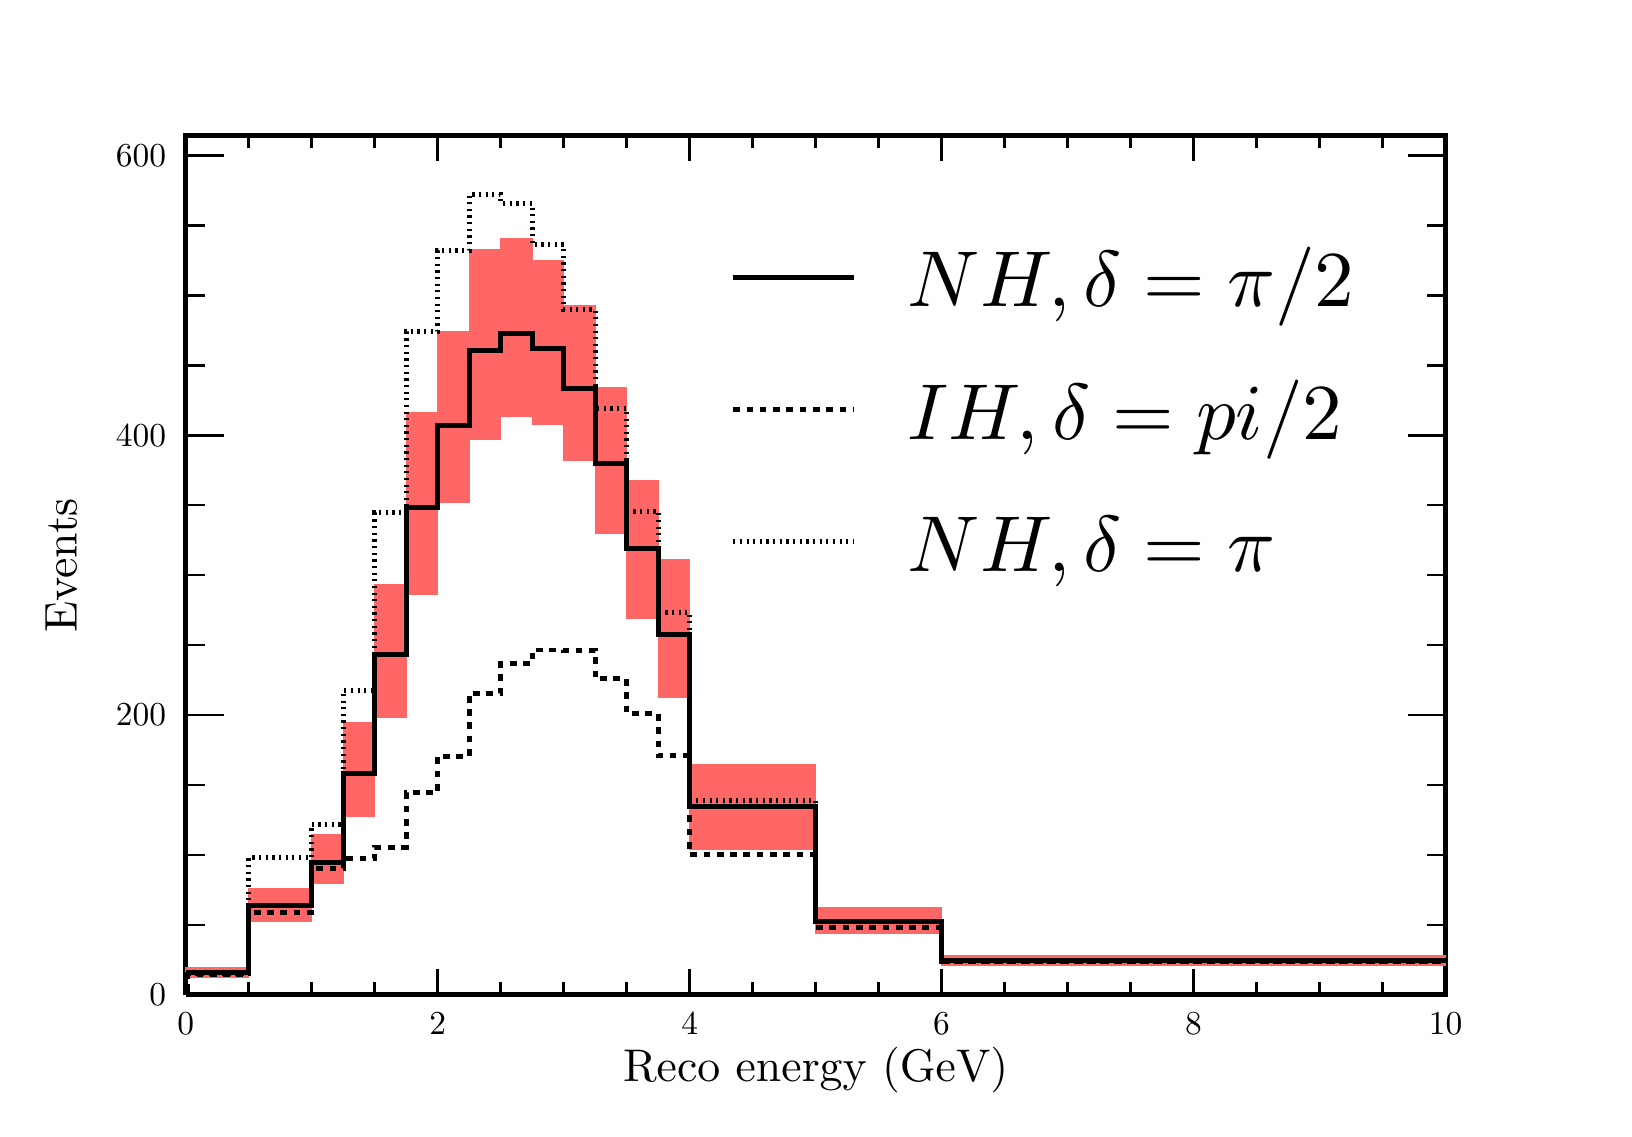
\begin{tikzpicture}
\pgfdeclareplotmark{cross} {
\pgfpathmoveto{\pgfpoint{-0.3\pgfplotmarksize}{\pgfplotmarksize}}
\pgfpathlineto{\pgfpoint{+0.3\pgfplotmarksize}{\pgfplotmarksize}}
\pgfpathlineto{\pgfpoint{+0.3\pgfplotmarksize}{0.3\pgfplotmarksize}}
\pgfpathlineto{\pgfpoint{+1\pgfplotmarksize}{0.3\pgfplotmarksize}}
\pgfpathlineto{\pgfpoint{+1\pgfplotmarksize}{-0.3\pgfplotmarksize}}
\pgfpathlineto{\pgfpoint{+0.3\pgfplotmarksize}{-0.3\pgfplotmarksize}}
\pgfpathlineto{\pgfpoint{+0.3\pgfplotmarksize}{-1.\pgfplotmarksize}}
\pgfpathlineto{\pgfpoint{-0.3\pgfplotmarksize}{-1.\pgfplotmarksize}}
\pgfpathlineto{\pgfpoint{-0.3\pgfplotmarksize}{-0.3\pgfplotmarksize}}
\pgfpathlineto{\pgfpoint{-1.\pgfplotmarksize}{-0.3\pgfplotmarksize}}
\pgfpathlineto{\pgfpoint{-1.\pgfplotmarksize}{0.3\pgfplotmarksize}}
\pgfpathlineto{\pgfpoint{-0.3\pgfplotmarksize}{0.3\pgfplotmarksize}}
\pgfpathclose
\pgfusepathqstroke
}
\pgfdeclareplotmark{cross*} {
\pgfpathmoveto{\pgfpoint{-0.3\pgfplotmarksize}{\pgfplotmarksize}}
\pgfpathlineto{\pgfpoint{+0.3\pgfplotmarksize}{\pgfplotmarksize}}
\pgfpathlineto{\pgfpoint{+0.3\pgfplotmarksize}{0.3\pgfplotmarksize}}
\pgfpathlineto{\pgfpoint{+1\pgfplotmarksize}{0.3\pgfplotmarksize}}
\pgfpathlineto{\pgfpoint{+1\pgfplotmarksize}{-0.3\pgfplotmarksize}}
\pgfpathlineto{\pgfpoint{+0.3\pgfplotmarksize}{-0.3\pgfplotmarksize}}
\pgfpathlineto{\pgfpoint{+0.3\pgfplotmarksize}{-1.\pgfplotmarksize}}
\pgfpathlineto{\pgfpoint{-0.3\pgfplotmarksize}{-1.\pgfplotmarksize}}
\pgfpathlineto{\pgfpoint{-0.3\pgfplotmarksize}{-0.3\pgfplotmarksize}}
\pgfpathlineto{\pgfpoint{-1.\pgfplotmarksize}{-0.3\pgfplotmarksize}}
\pgfpathlineto{\pgfpoint{-1.\pgfplotmarksize}{0.3\pgfplotmarksize}}
\pgfpathlineto{\pgfpoint{-0.3\pgfplotmarksize}{0.3\pgfplotmarksize}}
\pgfpathclose
\pgfusepathqfillstroke
}
\pgfdeclareplotmark{newstar} {
\pgfpathmoveto{\pgfqpoint{0pt}{\pgfplotmarksize}}
\pgfpathlineto{\pgfqpointpolar{44}{0.5\pgfplotmarksize}}
\pgfpathlineto{\pgfqpointpolar{18}{\pgfplotmarksize}}
\pgfpathlineto{\pgfqpointpolar{-20}{0.5\pgfplotmarksize}}
\pgfpathlineto{\pgfqpointpolar{-54}{\pgfplotmarksize}}
\pgfpathlineto{\pgfqpointpolar{-90}{0.5\pgfplotmarksize}}
\pgfpathlineto{\pgfqpointpolar{234}{\pgfplotmarksize}}
\pgfpathlineto{\pgfqpointpolar{198}{0.5\pgfplotmarksize}}
\pgfpathlineto{\pgfqpointpolar{162}{\pgfplotmarksize}}
\pgfpathlineto{\pgfqpointpolar{134}{0.5\pgfplotmarksize}}
\pgfpathclose
\pgfusepathqstroke
}
\pgfdeclareplotmark{newstar*} {
\pgfpathmoveto{\pgfqpoint{0pt}{\pgfplotmarksize}}
\pgfpathlineto{\pgfqpointpolar{44}{0.5\pgfplotmarksize}}
\pgfpathlineto{\pgfqpointpolar{18}{\pgfplotmarksize}}
\pgfpathlineto{\pgfqpointpolar{-20}{0.5\pgfplotmarksize}}
\pgfpathlineto{\pgfqpointpolar{-54}{\pgfplotmarksize}}
\pgfpathlineto{\pgfqpointpolar{-90}{0.5\pgfplotmarksize}}
\pgfpathlineto{\pgfqpointpolar{234}{\pgfplotmarksize}}
\pgfpathlineto{\pgfqpointpolar{198}{0.5\pgfplotmarksize}}
\pgfpathlineto{\pgfqpointpolar{162}{\pgfplotmarksize}}
\pgfpathlineto{\pgfqpointpolar{134}{0.5\pgfplotmarksize}}
\pgfpathclose
\pgfusepathqfillstroke
}
\definecolor{c}{rgb}{0.999,0.999,0.999};
\draw [color=c, fill=c] (0,0) rectangle (20,13.639);
\draw [color=c, fill=c] (2,1.3639) rectangle (18,12.2751);
\definecolor{c}{rgb}{0,0,0};
\draw [c,line width=1.8] (2,1.3639) -- (2,12.2751) -- (18,12.2751) -- (18,1.3639) -- (2,1.3639);
\definecolor{c}{rgb}{0.999,0.999,0.999};
\draw [color=c, fill=c] (2,1.3639) rectangle (18,12.2751);
\definecolor{c}{rgb}{0,0,0};
\draw [c,line width=1.8] (2,1.3639) -- (2,12.2751) -- (18,12.2751) -- (18,1.3639) -- (2,1.3639);
\draw [c,line width=1.8] (2,1.64385) -- (2.8,1.64385) -- (2.8,2.4955) -- (3.6,2.4955) -- (3.6,3.04067) -- (4,3.04067) -- (4,4.17002) -- (4.4,4.17002) -- (4.4,5.68074) -- (4.8,5.68074) -- (4.8,7.55117) -- (5.2,7.55117) -- (5.2,8.59541) --
 (5.6,8.59541) -- (5.6,9.54186) -- (6,9.54186) -- (6,9.75711) -- (6.4,9.75711) -- (6.4,9.57209) -- (6.8,9.57209) -- (6.8,9.0685) -- (7.2,9.0685) -- (7.2,8.10527) -- (7.6,8.10527) -- (7.6,7.03512) -- (8,7.03512) -- (8,5.93304) -- (8.4,5.93304) --
 (8.4,3.75508) -- (10,3.75508) -- (10,2.29637) -- (11.6,2.29637) -- (11.6,1.79751) -- (18,1.79751);
\draw [c,line width=0.9] (2,1.3639) -- (18,1.3639);
\draw [c,line width=0.9] (2,1.69123) -- (2,1.3639);
\draw [c,line width=0.9] (2.8,1.52756) -- (2.8,1.3639);
\draw [c,line width=0.9] (3.6,1.52756) -- (3.6,1.3639);
\draw [c,line width=0.9] (4.4,1.52756) -- (4.4,1.3639);
\draw [c,line width=0.9] (5.2,1.69123) -- (5.2,1.3639);
\draw [c,line width=0.9] (6,1.52756) -- (6,1.3639);
\draw [c,line width=0.9] (6.8,1.52756) -- (6.8,1.3639);
\draw [c,line width=0.9] (7.6,1.52756) -- (7.6,1.3639);
\draw [c,line width=0.9] (8.4,1.69123) -- (8.4,1.3639);
\draw [c,line width=0.9] (9.2,1.52756) -- (9.2,1.3639);
\draw [c,line width=0.9] (10,1.52756) -- (10,1.3639);
\draw [c,line width=0.9] (10.8,1.52756) -- (10.8,1.3639);
\draw [c,line width=0.9] (11.6,1.69123) -- (11.6,1.3639);
\draw [c,line width=0.9] (12.4,1.52756) -- (12.4,1.3639);
\draw [c,line width=0.9] (13.2,1.52756) -- (13.2,1.3639);
\draw [c,line width=0.9] (14,1.52756) -- (14,1.3639);
\draw [c,line width=0.9] (14.8,1.69123) -- (14.8,1.3639);
\draw [c,line width=0.9] (15.6,1.52756) -- (15.6,1.3639);
\draw [c,line width=0.9] (16.4,1.52756) -- (16.4,1.3639);
\draw [c,line width=0.9] (17.2,1.52756) -- (17.2,1.3639);
\draw [c,line width=0.9] (18,1.69123) -- (18,1.3639);
\draw [anchor=base] (2,0.859255) node[scale=1.20912, color=c, rotate=0]{0};
\draw [anchor=base] (5.2,0.859255) node[scale=1.20912, color=c, rotate=0]{2};
\draw [anchor=base] (8.4,0.859255) node[scale=1.20912, color=c, rotate=0]{4};
\draw [anchor=base] (11.6,0.859255) node[scale=1.20912, color=c, rotate=0]{6};
\draw [anchor=base] (14.8,0.859255) node[scale=1.20912, color=c, rotate=0]{8};
\draw [anchor=base] (18,0.859255) node[scale=1.20912, color=c, rotate=0]{10};
\draw (10,0.403714) node[scale=1.65459, color=c, rotate=0]{Reco energy (GeV)};
\draw [c,line width=0.9] (2,12.2751) -- (18,12.2751);
\draw [c,line width=0.9] (2,11.9477) -- (2,12.2751);
\draw [c,line width=0.9] (2.8,12.1114) -- (2.8,12.2751);
\draw [c,line width=0.9] (3.6,12.1114) -- (3.6,12.2751);
\draw [c,line width=0.9] (4.4,12.1114) -- (4.4,12.2751);
\draw [c,line width=0.9] (5.2,11.9477) -- (5.2,12.2751);
\draw [c,line width=0.9] (6,12.1114) -- (6,12.2751);
\draw [c,line width=0.9] (6.8,12.1114) -- (6.8,12.2751);
\draw [c,line width=0.9] (7.6,12.1114) -- (7.6,12.2751);
\draw [c,line width=0.9] (8.4,11.9477) -- (8.4,12.2751);
\draw [c,line width=0.9] (9.2,12.1114) -- (9.2,12.2751);
\draw [c,line width=0.9] (10,12.1114) -- (10,12.2751);
\draw [c,line width=0.9] (10.8,12.1114) -- (10.8,12.2751);
\draw [c,line width=0.9] (11.6,11.9477) -- (11.6,12.2751);
\draw [c,line width=0.9] (12.4,12.1114) -- (12.4,12.2751);
\draw [c,line width=0.9] (13.2,12.1114) -- (13.2,12.2751);
\draw [c,line width=0.9] (14,12.1114) -- (14,12.2751);
\draw [c,line width=0.9] (14.8,11.9477) -- (14.8,12.2751);
\draw [c,line width=0.9] (15.6,12.1114) -- (15.6,12.2751);
\draw [c,line width=0.9] (16.4,12.1114) -- (16.4,12.2751);
\draw [c,line width=0.9] (17.2,12.1114) -- (17.2,12.2751);
\draw [c,line width=0.9] (18,11.9477) -- (18,12.2751);
\draw [c,line width=0.9] (2,1.3639) -- (2,12.2751);
\draw [c,line width=0.9] (2.48,1.3639) -- (2,1.3639);
\draw [c,line width=0.9] (2.24,2.25207) -- (2,2.25207);
\draw [c,line width=0.9] (2.24,3.14024) -- (2,3.14024);
\draw [c,line width=0.9] (2.24,4.02841) -- (2,4.02841);
\draw [c,line width=0.9] (2.48,4.91657) -- (2,4.91657);
\draw [c,line width=0.9] (2.24,5.80474) -- (2,5.80474);
\draw [c,line width=0.9] (2.24,6.69291) -- (2,6.69291);
\draw [c,line width=0.9] (2.24,7.58108) -- (2,7.58108);
\draw [c,line width=0.9] (2.48,8.46925) -- (2,8.46925);
\draw [c,line width=0.9] (2.24,9.35742) -- (2,9.35742);
\draw [c,line width=0.9] (2.24,10.2456) -- (2,10.2456);
\draw [c,line width=0.9] (2.24,11.1338) -- (2,11.1338);
\draw [c,line width=0.9] (2.48,12.0219) -- (2,12.0219);
\draw [c,line width=0.9] (2.48,12.0219) -- (2,12.0219);
\draw [anchor= east] (1.9,1.3639) node[scale=1.20912, color=c, rotate=0]{0};
\draw [anchor= east] (1.9,4.91657) node[scale=1.20912, color=c, rotate=0]{200};
\draw [anchor= east] (1.9,8.46925) node[scale=1.20912, color=c, rotate=0]{400};
\draw [anchor= east] (1.9,12.0219) node[scale=1.20912, color=c, rotate=0]{600};
\draw (0.416,6.81948) node[scale=1.65459, color=c, rotate=90]{Events};
\draw [c,line width=0.9] (18,1.3639) -- (18,12.2751);
\draw [c,line width=0.9] (17.52,1.3639) -- (18,1.3639);
\draw [c,line width=0.9] (17.76,2.25207) -- (18,2.25207);
\draw [c,line width=0.9] (17.76,3.14024) -- (18,3.14024);
\draw [c,line width=0.9] (17.76,4.02841) -- (18,4.02841);
\draw [c,line width=0.9] (17.52,4.91657) -- (18,4.91657);
\draw [c,line width=0.9] (17.76,5.80474) -- (18,5.80474);
\draw [c,line width=0.9] (17.76,6.69291) -- (18,6.69291);
\draw [c,line width=0.9] (17.76,7.58108) -- (18,7.58108);
\draw [c,line width=0.9] (17.52,8.46925) -- (18,8.46925);
\draw [c,line width=0.9] (17.76,9.35742) -- (18,9.35742);
\draw [c,line width=0.9] (17.76,10.2456) -- (18,10.2456);
\draw [c,line width=0.9] (17.76,11.1338) -- (18,11.1338);
\draw [c,line width=0.9] (17.52,12.0219) -- (18,12.0219);
\draw [c,line width=0.9] (17.52,12.0219) -- (18,12.0219);
\definecolor{c}{rgb}{1,0.4,0.4};
\draw [color=c, fill=c] (2,1.58015) rectangle (2.8,1.7134);
\draw [color=c, fill=c] (2.8,2.29213) rectangle (3.6,2.71872);
\draw [color=c, fill=c] (3.6,2.78395) rectangle (4,3.39413);
\draw [color=c, fill=c] (4,3.62681) rectangle (4.4,4.82152);
\draw [color=c, fill=c] (4.4,4.88881) rectangle (4.8,6.57058);
\draw [color=c, fill=c] (4.8,6.44707) rectangle (5.2,8.76228);
\draw [color=c, fill=c] (5.2,7.61558) rectangle (5.6,9.7925);
\draw [color=c, fill=c] (5.6,8.41168) rectangle (6,10.8229);
\draw [color=c, fill=c] (6,8.70899) rectangle (6.4,10.9686);
\draw [color=c, fill=c] (6.4,8.60219) rectangle (6.8,10.6924);
\draw [color=c, fill=c] (6.8,8.15486) rectangle (7.2,10.1205);
\draw [color=c, fill=c] (7.2,7.21737) rectangle (7.6,9.06911);
\draw [color=c, fill=c] (7.6,6.1376) rectangle (8,7.89091);
\draw [color=c, fill=c] (8,5.13712) rectangle (8.4,6.88859);
\draw [color=c, fill=c] (8.4,3.20749) rectangle (10,4.28877);
\draw [color=c, fill=c] (10,2.14873) rectangle (11.6,2.46598);
\draw [color=c, fill=c] (11.6,1.73357) rectangle (18,1.86509);
\definecolor{c}{rgb}{0,0,0};
\draw [c,line width=1.8] (2,1.64385) -- (2.8,1.64385) -- (2.8,2.4955) -- (3.6,2.4955) -- (3.6,3.04067) -- (4,3.04067) -- (4,4.17002) -- (4.4,4.17002) -- (4.4,5.68074) -- (4.8,5.68074) -- (4.8,7.55117) -- (5.2,7.55117) -- (5.2,8.59541) --
 (5.6,8.59541) -- (5.6,9.54186) -- (6,9.54186) -- (6,9.75711) -- (6.4,9.75711) -- (6.4,9.57209) -- (6.8,9.57209) -- (6.8,9.0685) -- (7.2,9.0685) -- (7.2,8.10527) -- (7.6,8.10527) -- (7.6,7.03512) -- (8,7.03512) -- (8,5.93304) -- (8.4,5.93304) --
 (8.4,3.75508) -- (10,3.75508) -- (10,2.29637) -- (11.6,2.29637) -- (11.6,1.79751) -- (18,1.79751);
\draw [c,dash pattern=on 2.40pt off 2.40pt ,line width=1.8] (2.02865,1.39255) -- (2.02865,1.61977) -- (2.8,1.61977) -- (2.8,2.41107) -- (3.6,2.41107) -- (3.6,2.96834) -- (4,2.96834) -- (4,3.09236) -- (4.4,3.09236) -- (4.4,3.23892) -- (4.8,3.23892) --
 (4.8,3.933) -- (5.2,3.933) -- (5.2,4.396) -- (5.6,4.396) -- (5.6,5.1953) -- (6,5.1953) -- (6,5.56987) -- (6.4,5.56987) -- (6.4,5.74248) -- (6.8,5.74248) -- (6.8,5.73905) -- (7.2,5.73905) -- (7.2,5.37435) -- (7.6,5.37435) -- (7.6,4.93637) --
 (8,4.93637) -- (8,4.39961) -- (8.4,4.39961) -- (8.4,3.14541) -- (10,3.14541) -- (10,2.21288) -- (11.6,2.21288) -- (11.6,1.78649) -- (18,1.78649);
\draw [c,dash pattern=on 0.80pt off 1.60pt ,line width=1.8] (2.02865,1.39255) -- (2.02865,1.63661) -- (2.8,1.63661) -- (2.8,3.10507) -- (3.6,3.10507) -- (3.6,3.53228) -- (4,3.53228) -- (4,5.22798) -- (4.4,5.22798) -- (4.4,7.48346) -- (4.8,7.48346) --
 (4.8,9.78237) -- (5.2,9.78237) -- (5.2,10.8173) -- (5.6,10.8173) -- (5.6,11.5299) -- (6,11.5299) -- (6,11.4147) -- (6.4,11.4147) -- (6.4,10.8885) -- (6.8,10.8885) -- (6.8,10.0652) -- (7.2,10.0652) -- (7.2,8.81124) -- (7.6,8.81124) -- (7.6,7.50156)
 -- (8,7.50156) -- (8,6.22071) -- (8.4,6.22071) -- (8.4,3.82997) -- (10,3.82997) -- (10,2.29002) -- (11.6,2.29002) -- (11.6,1.79186) -- (18,1.79186);
\definecolor{c}{rgb}{1,1,1};
\draw [color=c, fill=c] (8.62464,6.27507) rectangle (17.3925,11.3181);
\definecolor{c}{rgb}{0,0,0};
\draw [anchor=base west] (10.8166,10.0993) node[scale=2.86371, color=c, rotate=0]{$NH, \delta = \pi/2$};
\draw [c,line width=1.8] (8.95344,10.4776) -- (10.4878,10.4776);
\draw [anchor=base west] (10.8166,8.41834) node[scale=2.86371, color=c, rotate=0]{$IH, \delta = pi/2$};
\draw [c,dash pattern=on 2.40pt off 2.40pt ,line width=1.8] (8.95344,8.79656) -- (10.4878,8.79656);
\draw [anchor=base west] (10.8166,6.73734) node[scale=2.86371, color=c, rotate=0]{$NH, \delta = \pi$};
\draw [c,dash pattern=on 0.80pt off 1.60pt ,line width=1.8] (8.95344,7.11557) -- (10.4878,7.11557);
\end{tikzpicture}
